% PIC: @ekyaaa
\chapter{Panduan Pengguna EVA Mobile (Pasien)}
\label{chap:eva-mobile}

\textbf{EVA Mobile} adalah aplikasi ponsel cerdas (\texttt{apps/eva\_mobile}) yang dirancang khusus sebagai ruang aman pendamping kesehatan mental 24/7 bagi pengguna dan pasien Generasi Z. Aplikasi ini memadukan pendamping kecerdasan buatan (\textit{EVA AI Companion}) yang empatik dan bebas stigma, skrining psikometrik mandiri berbasis bukti ilmiah, pencatatan jurnal emosi terenkripsi lokal, serta gerbang telekonseling langsung dengan psikolog berlisensi resmi.

\section{Onboarding, Tutorial, dan Beranda}

\subsection{Alur Registrasi dan Onboarding Pertama Kali}
Saat pertama kali mengunduh dan membuka EVA Mobile, pengguna disambut dengan layar \textit{Splash Onboarding} yang mengenalkan persona EVA serta komitmen privasi aplikasi.

\begin{steplist}
  \item Buka aplikasi EVA Mobile dan klik \textbf{Mulai Sekarang}.
  \item Pilih \textbf{Daftar Akun} pada halaman login. Masukkan Nama Panggilan (\textit{display name}), Email aktif, serta Kata Sandi yang aman.
  \item Setujui \textbf{Syarat Ketentuan \& Kebijakan Privasi}. Pengguna diingatkan bahwa EVA adalah asisten pendamping emosi suportif dan bukan pengganti instalasi gawat darurat psikiatri.
  \item Ikuti tur panduan interaktif singkat mengenai navigasi bilah bawah (\textit{Bottom Navigation Bar}) yang terdiri dari: \textbf{Beranda}, \textbf{Curhat AI}, \textbf{Diari}, \textbf{Cari Psikolog}, dan \textbf{Profil/Pengaturan}.
\end{steplist}

\subsection{Antarmuka Beranda Utama (\textit{Dashboard})}
Halaman Beranda dirancang dengan tata letak visual yang menenangkan (palet Periwinkle dan Slate lembut), menyajikan ringkasan kondisi emosional pengguna hari ini tanpa rasa intimidasi:
\begin{itemize}[leftmargin=1.4em]
  \item \textbf{Header Sapaan Emosional}: Menampilkan nama panggilan pengguna, saldo \textbf{EVA Coin}, dan indikator suasana hati terkini.
  \item \textbf{Kartu Pintasan Curhat Cepat}: Tombol satu sentuhan untuk langsung memulai sesi panggilan suara interaktif (\textit{Voice Call}) bersama EVA.
  \item \textbf{Kartu Progres Perawatan Diri (\textit{0/3 -- 3/3 Selesai})}: Pelacak gamifikasi harian non-kompetitif dengan bilah progres 3 segmen untuk tiga rutinitas terapeutik (\textit{Sesi Curhat Bersama Eva}, \textit{Refleksi Jurnal Harian}, dan \textit{Latihan Relaksasi \& Koping}).
  \item \textbf{Status Skrining Emosional}: Menampilkan skor DASS-21 terakhir dan rekomendasi aksi perawatan diri.
\end{itemize}

\uifigure[0.38\textwidth]{mobile/01_onboarding_beranda.png}{Tampilan Beranda Utama EVA Mobile (\texttt{/\#/home})}{fig:mobile-home}

\section{EVA AI Chat dan Voice Call}

\subsection{Percakapan Suara Real-Time (\textit{Interactive Voice Call})}
Fitur unggulan EVA Mobile adalah percakapan suara langsung dengan latensi sangat rendah, memungkinkan pengguna berbicara secara natural layaknya mengobrol dengan sahabat terpercaya di jam-jam rawan malam hari (\textit{The 2 AM Crisis}).

\begin{steplist}
  \item Ketuk ikon mikrofon besar pada bilah navigasi atau tombol \textbf{Mulai Curhat Suara} di Beranda.
  \item Izinkan akses mikrofon perangkat saat sistem meminta izin audio pertama kali.
  \item Mulailah berbicara secara alami. Indikator bola energi (\textit{Orb Animation}) akan berekspresi secara dinamis merespons intonasi dan isi cerita pengguna.
  \item EVA merespons menggunakan sintesis suara ekspresif berbahasa Indonesia yang empatik, hangat, dan tanpa penghakiman.
  \item Ketuk tombol merah \textbf{Akhiri Sesi} kapan saja untuk menutup percakapan suara dan menyimpan rangkuman emosional.
\end{steplist}

\callouttip{Kualitas Audio Percakapan}{Gunakan earphone atau mikrofon bawaan di ruangan yang tenang agar modul Speech-to-Text dapat menangkap cerita Anda dengan artikulasi terbaik.}

\subsection{Safety Gate dan Dukungan Darurat Saat Terdeteksi Risiko Bunuh Diri}
Sistem dilengkapi modul \textbf{AI Safety Gate} deterministik yang memantau transkrip percakapan dan kondisi emosional pengguna secara \textit{real-time}:
\begin{itemize}[leftmargin=1.4em]
  \item \textbf{Deteksi Otomatis Saat Panggilan Berjalan}: Apabila pengguna mengucapkan indikasi bahaya diri atau niat bunuh diri (misalnya \textit{``Aku mau bunuh diri''}), panggilan suara bersama EVA \textbf{tidak langsung terputus}, melainkan tetap berlanjut secara empatik sambil menampilkan kartu peringatan merah muda \textbf{Dukungan Darurat Tersedia} dengan pesan \textit{``Panggilan EVA tetap berlanjut. Kamu tidak sendirian.''}.
  \item \textbf{Akses Bantuan Seketika di Layar Voice Call}: Kartu tersebut langsung menyediakan informasi layanan resmi \textbf{Hotline Dinkes (WhatsApp 0813-8007-3120) / Kemenkes 119 ext 8} beserta empat tombol aksi cepat satu sentuhan:
  \begin{enumerate}[leftmargin=1.4em]
    \item \textbf{Hotline 119 / LISA}: Menghubungkan langsung ke layanan krisis psikologis resmi.
    \item \textbf{Latihan Napas}: Membuka sesi stabilisasi pernapasan terpandu secara langsung untuk membantu menurunkan kepanikan akut.
    \item \textbf{WA Dinkes DKI}: Membuka percakapan WhatsApp darurat layanan kesehatan jiwa daerah (\texttt{0813-8007-3120}).
    \item \textbf{Orang Terdekat}: Menghubungi kontak darurat pribadi (\textit{Trusted Contact}) yang telah didaftarkan pengguna.
  \end{enumerate}
\end{itemize}

\uifigure[0.34\textwidth]{mobile/08_dukungan_darurat_in_call.jpg}{Kartu Dukungan Darurat Tersedia Saat Terdeteksi Risiko Bunuh Diri pada Voice Call}{fig:mobile-in-call-emergency}

\uifigure[0.38\textwidth]{mobile/02_ai_voice_call.png}{Layar Sesi Panggilan Suara Interaktif (AI Voice Call)}{fig:mobile-voice}

\section{Local Selective Memory dan Consent Sharing}

\subsection{Kedaulatan Data dengan SQLCipher (\textit{Local Memory})}
Berbeda dengan kecerdasan buatan konvensional yang menyimpan seluruh log riwayat obrolan di server awan secara terbuka, EVA Ecosystem mengimplementasikan prinsip \textbf{Kedaulatan Data Pasien (\textit{Patient Data Sovereignty})}:
\begin{itemize}[leftmargin=1.4em]
  \item Seluruh memori percakapan jangka panjang (\textit{Long-Term Memory/LTM}) dienkripsi menggunakan kunci derivasi perangkat tingkat militer melalui mesin basis data \textbf{SQLCipher}.
  \item Pengguna dapat memeriksa memori apa saja yang diingat oleh EVA melalui menu \textbf{Pengaturan Privasi \& Memori AI}.
  \item \textbf{Penghapusan Selektif (\textit{Selective Deletion})}: Pengguna memiliki hak mutlak untuk menghapus poin-poin memori spesifik atau mereset seluruh riwayat ingatan dengan satu kali klik.
\end{itemize}

\subsection{Mekanisme Izin Berbagi Data (\textit{Consent Switch})}
Riwayat obrolan dan grafik emosi pengguna \textbf{tidak pernah dibagikan kepada psikolog atau pihak ketiga mana pun secara default}. 

\calloutwarn{Kendali Penuh di Tangan Pasien}{Sebelum sesi telekonsultasi dengan psikolog dimulai, aplikasi menampilkan sakelar persetujuan (\textit{Consent Toggle}). Hanya jika sakelar ini diaktifkan oleh pasien, psikolog mitra dapat melihat ringkasan klinis DASS-21 dan pemicu stres utama untuk keperluan terapi.}

\uifigure[0.38\textwidth]{mobile/07_pengaturan_privasi.png}{Pengaturan Privasi, Akun, dan Personalisasi Avatar}{fig:mobile-settings}

\section{Skrining DASS-21 dan Monitoring Grafik}

\subsection{Pelaksanaan Skrining Mandiri DASS-21}
Aplikasi menyediakan instrumen psikometri baku \textbf{Depression Anxiety Stress Scale (DASS-21)} yang telah divalidasi secara klinis untuk populasi Indonesia.
\begin{steplist}
  \item Akses tab \textbf{Skrining} dari menu bawah atau kartu rekomendasi Beranda.
  \item Jawab 21 butir pertanyaan sederhana mengenai kondisi yang dialami dalam 7 hari terakhir menggunakan skala 0 (\textit{Tidak Pernah}) hingga 3 (\textit{Sangat Sering}).
  \item Klik \textbf{Kirim \& Lihat Hasil} untuk memproses skor secara instan.
\end{steplist}

\subsection{Interpretasi Skor dan Rekomendasi Klinis}
Hasil skrining dipetakan ke dalam tiga dimensi terpisah dengan lima tingkat keparahan:
\begin{itemize}[leftmargin=1.4em]
  \item \textbf{Depresi (\textit{Depression})}: Mengukur tingkat disforia, keputusasaan, dan ketiadaan minat hidup.
  \item \textbf{Kecemasan (\textit{Anxiety})}: Mengukur respons rangsangan otonom, ketegangan fisik, dan rasa panik situasional.
  \item \textbf{Stres (\textit{Stress})}: Mengukur ketegangan non-spesifik, iritabilitas, dan kesulitan relaksasi.
\end{itemize}

\begin{table}[htbp]
  \centering
  \caption{Norma Tingkat Keparahan Skrining DASS-21 di EVA Mobile}
  \label{tab:dass-norms}
  \small
  \begin{tabularx}{\textwidth}{@{}lccccX@{}}
    \toprule
    \textbf{Dimensi} & \textbf{Normal} & \textbf{Ringan} & \textbf{Sedang} & \textbf{Parah} & \textbf{Sangat Parah} \\
    \midrule
    \textbf{Depresi} & 0--9 & 10--13 & 14--20 & 21--27 & $\ge 28$ (Rekomendasi Rujukan Klinis) \\
    \textbf{Kecemasan} & 0--7 & 8--9 & 10--14 & 15--19 & $\ge 20$ (Rekomendasi Rujukan Klinis) \\
    \textbf{Stres} & 0--14 & 15--18 & 19--25 & 26--33 & $\ge 34$ (Rekomendasi Rujukan Klinis) \\
    \bottomrule
  \end{tabularx}
\end{table}

Pengguna dapat memantau riwayat fluktuasi skor dari minggu ke minggu melalui diagram garis interaktif untuk melihat progres pemulihan.

\uifigure[0.38\textwidth]{mobile/04_skrining_dass21.png}{Halaman Skrining Mandiri DASS-21 Klinis}{fig:mobile-screening}

\section{Diary, Gamifikasi Perawatan Diri, dan Coping Missions}

\subsection{Diari Emosi AI (\textit{Smart Emotional Journaling})}
Modul Diari memungkinkan pengguna menuliskan refleksi harian secara bebas:
\begin{itemize}[leftmargin=1.4em]
  \item Pengguna memilih ikon penanda suasana hati (\textit{Mood Sticker}) dan menuliskan curahan hati atau catatan peristiwa penting hari itu.
  \item Mesin Natural Language Processing (NLP) EVA menganalisis tulisan pengguna dan menyematkan tag kognitif otomatis (misalnya: \textit{Overthinking, Burnout Akademik, Kesepian, Gratitude}).
  \item Di akhir pekan, aplikasi menyusun \textbf{Sintesis Diari Mingguan} yang merangkum pola pemicu emosi dan menawarkan afirmasi positif.
\end{itemize}

\uifigure[0.38\textwidth]{mobile/03_diary_coping.png}{Diari Emosi AI dan Refleksi Pikiran}{fig:mobile-diary}

\subsection{Gamifikasi Perawatan Diri Harian (\textit{Daily Self-Care Progress})}
EVA Mobile menerapkan gamifikasi suportif non-kompetitif pada kartu \textbf{Perawatan Diri} di Beranda (tanpa hukuman \textit{streak} atau papan peringkat yang memicu rasa bersalah) untuk menjaga konsistensi kebiasaan baik pengguna:
\begin{itemize}[leftmargin=1.4em]
  \item \textbf{Progres 3 Segmen (\texttt{0/3} hingga \texttt{3/3 Selesai})}: Menampilkan bilah progres bertahap dengan persentase pencapaian harian (\texttt{0\%}--\texttt{100\%}) dan pesan motivasi adaptif pada setiap langkah penyelesaian.
  \item \textbf{Tiga Rutinitas Terapeutik Harian}:
  \begin{enumerate}[leftmargin=1.4em]
    \item \textbf{Sesi Curhat Bersama Eva}: Mencatat keterlibatan pengguna dalam dialog suara atau teks hari ini.
    \item \textbf{Refleksi Jurnal Harian}: Otomatis tercentang saat pengguna membaca atau menyusun rangkuman dan pola emosi harian.
    \item \textbf{Latihan Relaksasi \& Koping}: Otomatis tercentang saat pengguna menyelesaikan minimal satu latihan dari katalog \textbf{Panduan Ketenangan}.
  \end{enumerate}
\end{itemize}

\uifigure[0.34\textwidth]{mobile/09_gamifikasi_perawatan_diri.png}{Kartu Gamifikasi Perawatan Diri Harian (\texttt{2/3 Selesai}) di Beranda EVA Mobile}{fig:mobile-gamifikasi-progress}

\subsection{Panduan Ketenangan dan Misi Coping Interaktif (\textit{CBT \& Mindfulness})}
Melalui halaman \textbf{Latihan Coping \& Relaksasi} (\texttt{/coping}), pengguna dapat mengikuti alur latihan terstruktur: memilih kartu latihan $\rightarrow$ membaca panduan singkat pada dialog tutorial awal $\rightarrow$ memulai sesi interaktif $\rightarrow$ sistem mencatat penyelesaian ke progres harian serta menyinkronkan status rekomendasi. Saat ini tersedia enam modul koping aktif yang dirangkum pada Tabel~\ref{tab:coping-catalog}:

\begin{table}[htbp]
  \centering
  \caption{Katalog Modul Panduan Ketenangan dan Gamifikasi Coping di EVA Mobile}
  \label{tab:coping-catalog}
  \small
  \begin{tabularx}{\textwidth}{@{}p{4.3cm}p{2.3cm}p{2.3cm}X@{}}
    \toprule
    \textbf{Nama Modul} & \textbf{Kategori} & \textbf{Durasi} & \textbf{Mekanika \& Fokus Latihan} \\
    \midrule
    \textbf{Latihan Pernapasan Terpandu} & Mindfulness & Sekitar 1 Menit & Pengalaman visual imersif: fase persiapan 4 detik, 4 siklus tarik--hembus (4 detik tarik / 4 detik hembus), penutup 4 detik, animasi gelombang napas, partikel, dan efek sentuhan (\textit{touch ripple}). \\
    \addlinespace[4pt]
    \textbf{Teknik Grounding 5-4-3-2-1} & CBT & 5 Menit & Panduan kesadaran panca indra (5 dilihat, 4 disentuh, 3 didengar, 2 dicium, 1 dirasakan) untuk meredakan kecemasan akut. \\
    \addlinespace[4pt]
    \textbf{Catatan Syukur Harian} & Refleksi & 3 Menit & Refleksi mikro hal-hal positif harian guna menyeimbangkan bias pikiran negatif. \\
    \addlinespace[4pt]
    \textbf{Metode Notice and Name} & CBT & 4 Menit & Latihan menamai dan mengambil jarak dari pikiran mengganggu (\textit{cognitive defusion}). \\
    \addlinespace[4pt]
    \textbf{Metode Stop-Think-Go} & CBT & 5 Menit & Langkah terarah berhenti sejenak, menimbang opsi, dan menentukan solusi bertahap saat beban menumpuk. \\
    \addlinespace[4pt]
    \textbf{Jalan Santai Mindful} & Fisik \& Gerak & 10 Menit & Aktivitas gerak ringan berkesadaran penuh untuk melepaskan ketegangan fisik dan mental. \\
    \bottomrule
  \end{tabularx}
\end{table}

\begin{figure}[H]
  \centering
  \begin{minipage}[t]{0.31\textwidth}
    \centering
    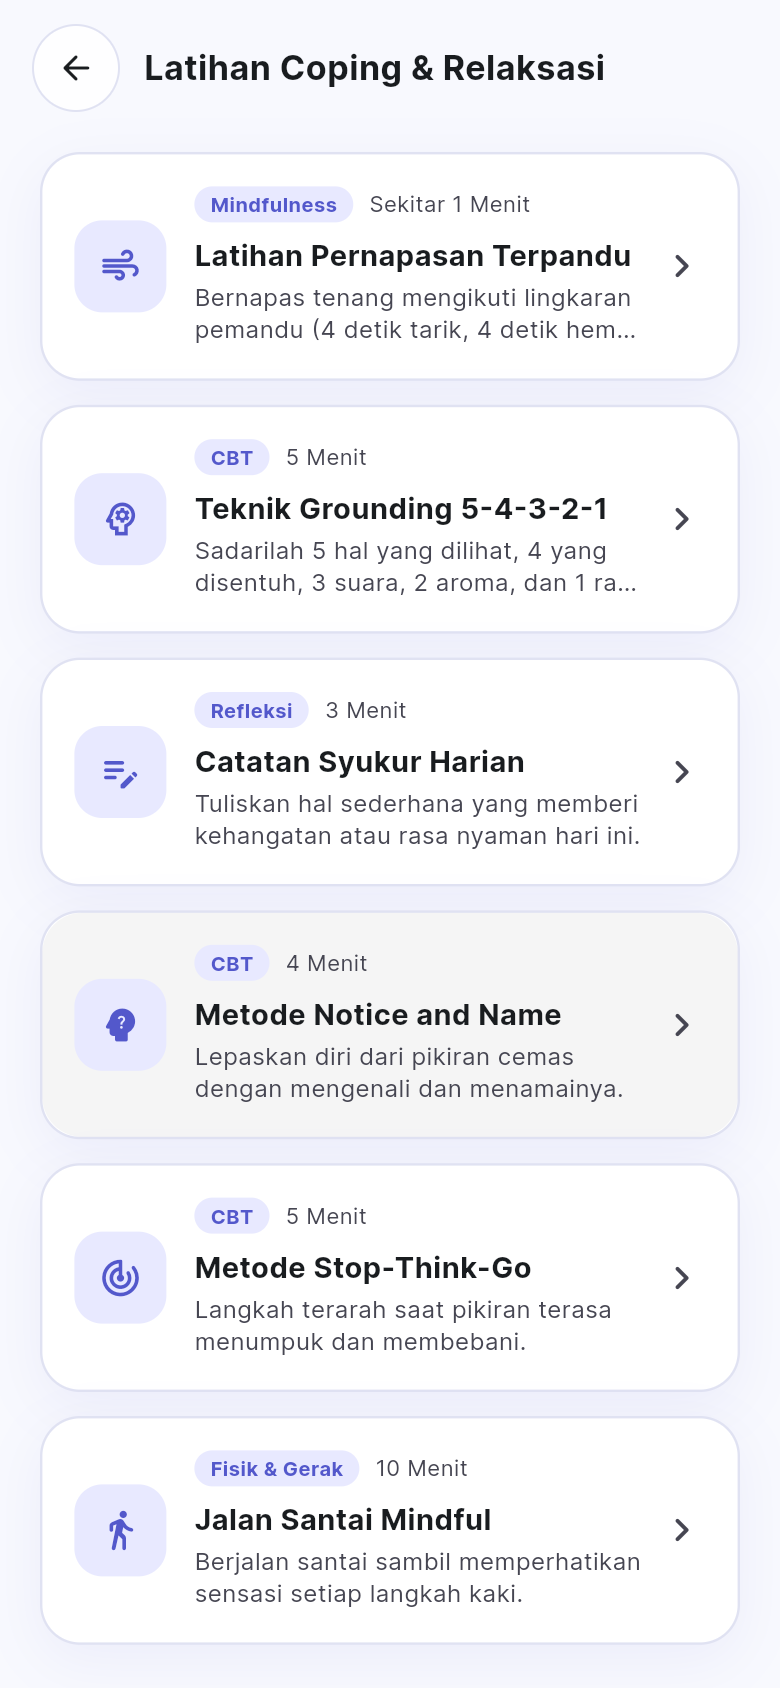
\includegraphics[width=\textwidth]{figures/mobile/10_panduan_ketenangan_katalog.png}
    \caption{Katalog 6 Modul Latihan Coping \& Relaksasi (\texttt{/coping})}
    \label{fig:mobile-coping-catalog}
  \end{minipage}\hfill
  \begin{minipage}[t]{0.31\textwidth}
    \centering
    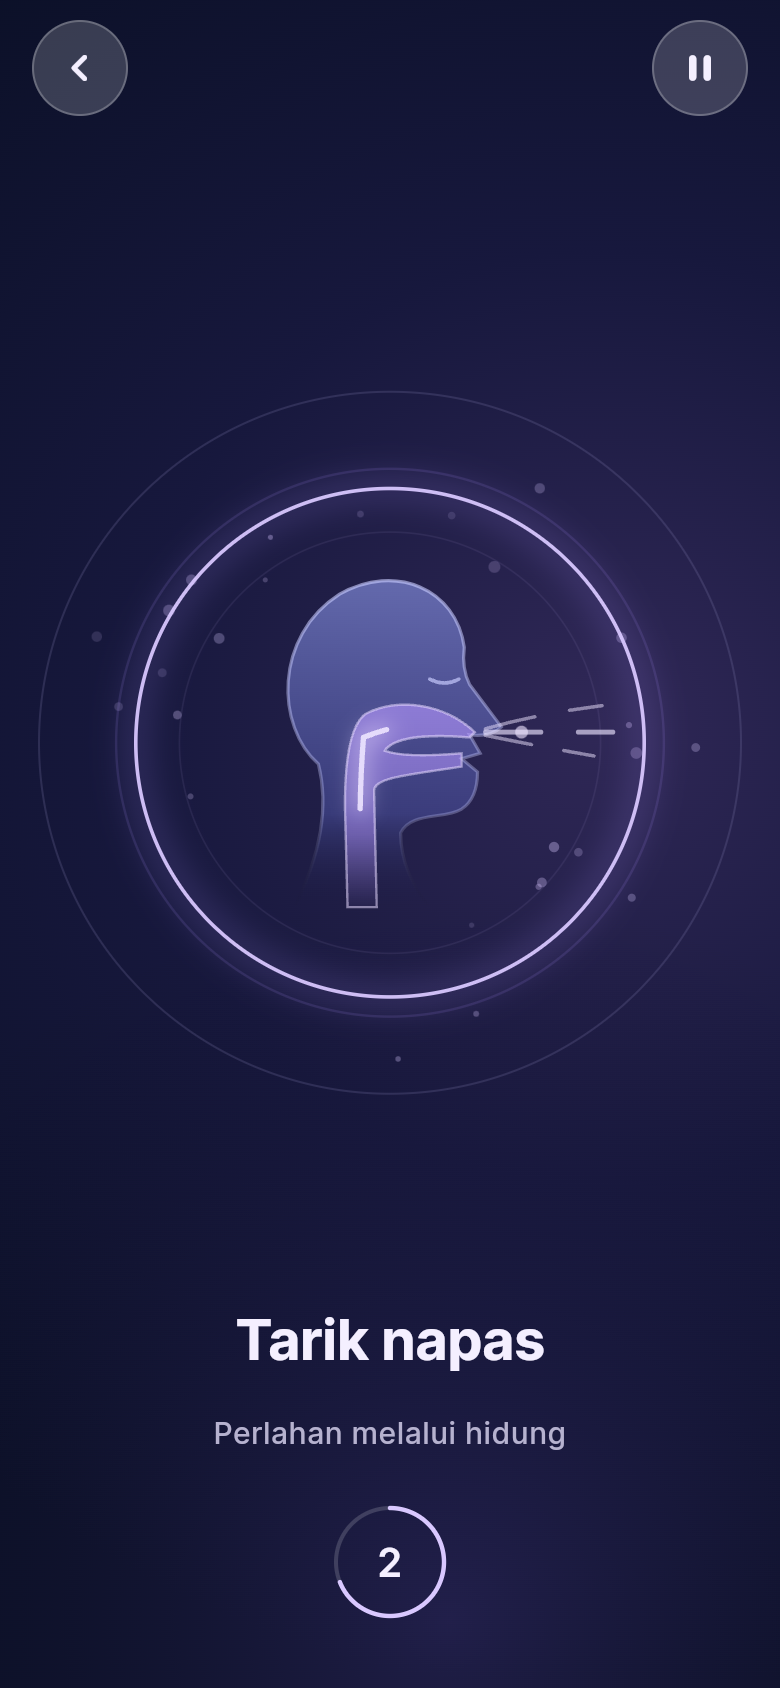
\includegraphics[width=\textwidth]{figures/mobile/11_latihan_pernapasan.png}
    \caption{Visual Interaktif Latihan Pernapasan Terpandu}
    \label{fig:mobile-breathing}
  \end{minipage}\hfill
  \begin{minipage}[t]{0.31\textwidth}
    \centering
    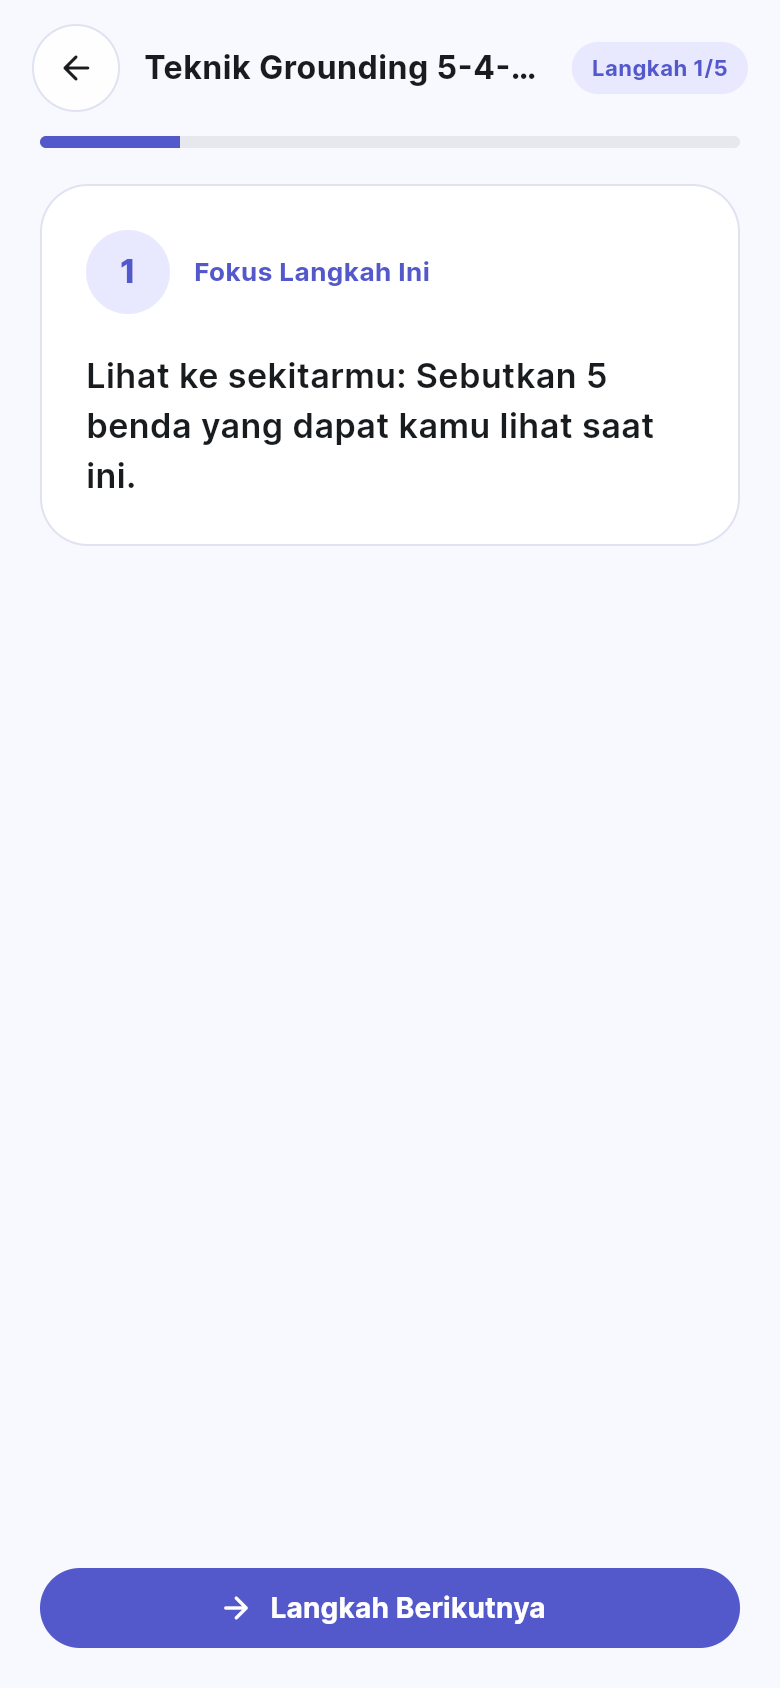
\includegraphics[width=\textwidth]{figures/mobile/12_teknik_grounding_54321.png}
    \caption{Modul Interaktif Teknik Grounding 5-4-3-2-1}
    \label{fig:mobile-grounding}
  \end{minipage}
\end{figure}

\uifigure[0.34\textwidth]{mobile/06_quest_monitoring.png}{Pemantauan Ritme \& Tren Emosional Harian}{fig:mobile-quest}

\section{EVA Coin (Saldo, Paket, Top-up, dan Riwayat)}

\subsection{Sistem Mata Uang Internal EVA Coin}
\textbf{EVA Coin} adalah mata uang virtual internal yang digunakan untuk memesan sesi konsultasi telekonseling dengan psikolog mitra berlisensi resmi:
\begin{itemize}[leftmargin=1.4em]
  \item Nilai konversi koin terstandar (\textbf{1 Koin = Rp 1.000}).
  \item Biaya sesi telekonseling 30 menit berkisar antara 50 hingga 150 EVA Coin, bergantung pada tingkat level pengalaman psikolog (Junior, Reguler, atau Senior).
\end{itemize}

\subsection{Cara Melakukan Top-up Saldo via QRIS}
\begin{steplist}
  \item Buka halaman \textbf{Dompet \& Koin} melalui header Beranda atau menu Profil.
  \item Pilih paket koin yang diinginkan (Tersedia paket 50, 100, 200, atau 500 koin).
  \item Pilih metode pembayaran instan \textbf{QRIS (Midtrans Sandbox/Production)}.
  \item Kode QRIS akan muncul di layar. Pindai menggunakan aplikasi m-Banking atau dompet digital (GoPay, OVO, Dana, ShopeePay).
  \item Setelah pembayaran berhasil, webhook Midtrans secara otomatis memverifikasi transaksi dan saldo koin langsung bertambah seketika.
\end{steplist}

\section{Konsultasi Psikolog dan Sesi Video Call}

\subsection{Mencari dan Memilih Psikolog Mitra}
Saat pengguna membutuhkan pertolongan klinis mendalam dari tenaga profesional manusia:
\begin{steplist}
  \item Buka tab \textbf{Cari Psikolog} pada bilah navigasi bawah.
  \item Gunakan filter pencarian berdasarkan fokus permasalahan (\textit{Keluarga, Depresi, Karier, Hubungan Interpersonal}), tarif koin, atau tingkat level psikolog.
  \item Klik kartu profil psikolog untuk melihat nomor STR/SIPP terverifikasi, ulasan bintang dari pasien lain, riwayat pendidikan, dan kalender ketersediaan jadwal.
\end{steplist}

\subsection{Pemesanan Jadwal dan Pelaksanaan Video Call}
\begin{steplist}
  \item Pilih tanggal dan slot waktu praktik yang tersedia (durasi 30 menit).
  \item Konfirmasi pembayaran menggunakan saldo EVA Coin dan tentukan izin pembagian rekam ringkasan emosi (\textit{Consent Toggle}).
  \item Pada waktu yang telah dijadwalkan, tombol \textbf{Masuk Ruang Sesi} akan aktif pada halaman jadwal.
  \item Sesi telekonseling berjalan melalui sambungan video WebRTC terenkripsi \textit{peer-to-peer}.
  \item Selesai sesi, pasien dapat memberikan penilaian bintang (1 hingga 5) serta ulasan kualitatif yang membantu menjaga transparansi mutu layanan.
\end{steplist}

\section{Layanan Darurat Krisis}

Ketika pengguna berada dalam ancaman bahaya fisik, dorongan bunuh diri akut, atau tindak kekerasan seketika, EVA Mobile menyediakan akses cepat \textbf{SafetyNet 24/7} (baik melalui halaman darurat khusus maupun kartu \textbf{Dukungan Darurat Tersedia} yang muncul langsung saat Voice Call):
\begin{itemize}[leftmargin=1.4em]
  \item \textbf{Hotline Nasional 119 ext 8 / LISA}: Panggilan satu sentuhan ke layanan konseling dan gawat darurat kesehatan jiwa Kementerian Kesehatan RI atau nomor darurat nasional (112).
  \item \textbf{WA Dinkes DKI (\texttt{0813-8007-3120})}: Akses pesan cepat WhatsApp untuk layanan konsultasi krisis kesehatan jiwa daerah.
  \item \textbf{Notifikasi Orang Terdekat (\textit{Trusted Contact})}: Mengirimkan sinyal darurat dan tautan bantuan kepada kontak terpercaya yang telah didaftarkan pengguna sebelumnya.
  \item \textbf{Panduan Latihan Napas Stabilisasi}: Akses langsung ke latihan pernapasan terpandu untuk menenangkan respons panik sambil menunggu pertolongan.
\end{itemize}

\uifigure[0.38\textwidth]{mobile/05_safetynet_krisis.png}{Protokol Bantuan Darurat dan Hotline Krisis 24/7}{fig:mobile-safety}
